\documentclass[tikz,convert={outext=.png}]{standalone}
\begin{document}
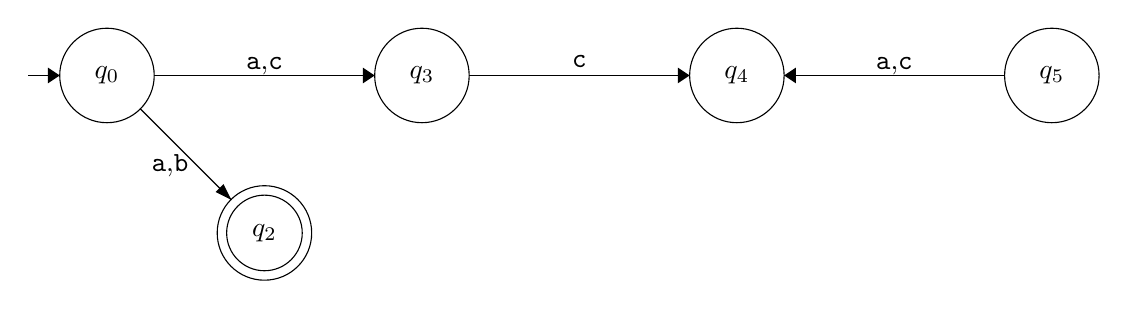
\begin{tikzpicture}[scale=0.2]
\tikzstyle{every node}+=[inner sep=0pt]
\draw [black] (-5,0) -- (-3,0);
\fill [black] (-3,0) -- (-3.75,-.5) -- (-3.75,.5);
\draw [black] (0,0) circle (3);
\draw (0,0) node {$q_0$};

\draw (10,0) node [above] {{\tt a},{\tt c}};
\draw [black] (3,0) -- (17,0);
\fill [black] (17,0) -- (16.25,-.5) -- (16.25,.5);
\draw [black] (20,0) circle (3);
\draw (20,0) node {$q_3$};

\draw (30,.5) node [above] {{\tt c}};
\draw [black] (23,0) -- (37,0);
\fill [black] (37,0) -- (36.25,-.5) -- (36.25,.5);
\draw [black] (40,0) circle (3);
\draw (40,0) node {$q_4$};

\draw (50,0) node [above] {{\tt a},{\tt c}};
\draw [black] (43,0) -- (57,0);
\fill [black] (43,0) -- (43.75,-.5) -- (43.75,.5);
\draw [black] (60,0) circle (3);
\draw (60,0) node {$q_5$};

\draw (4, -5) node [below] {{\tt a},{\tt b}};
\draw [black] (2.1,-2.1) -- (7.9,-7.9);
\fill [black] (7.9,-7.9) -- (6.9,-7.4) -- (7.4,-6.9);
\draw [black] (10,-10) circle (3);
\draw [black] (10,-10) circle (2.4);
\draw (10,-10) node {$q_2$};
\end{tikzpicture}
\end{document}
